\chapter{Introduction}

Many-body effects are of great interest for modern physics and many aspects of this field have vital importance not only for fundamental research, but for effects encountered and used in daily life. The behavior of electrons in a crystal for example is such a problem. It is the basis for many properties of condensed matter, such as the differences between metal, insulators and semiconductors. It is therefore of fundamental concern for all kinds of electronic applications. In several cases, the underlying laws of such processes can only be resolved when considering many-body systems. An example is superconductivity in cuprates, where the process is dominated by long-range electric and magnetic interaction \cite{cuprates}. Such systems can not be calculated easily but require complex and time-consuming simulations, when treated numerically, since the complexity of such periodic quantum systems grows exponentially with size\cite{feynman}. Studying the real systems in contrast, i.e. solid crystals or other materials, is similarly complicated, because solid materials limit the control over the parameters. Quantities such as density or depth of the atomic potentials cannot easily be changed in one material, which makes understanding the internal mechanisms much harder. A promising field of research, that aims to overcoming all these problems, is quantum simulation with ultracold gases. 

In the recent years many techniques have been invented to cool, trap and store neutral atoms, using devices like magneto optical traps or optical dipole traps\cite{metcalf}, that give rise methods like evaporative cooling to produce degenerate Fermi gases or Bose-Einstein condensates. By manipulating laser beams it has become possible to create potential landscapes, that emulate structures in solid crystals and allows to shape the Hamiltonian of such systems. They can be designed to resemble those proposed in models of condensed matter physics and the respective parameters can be controlled with high precision \cite{bloch}. One of the first experiments for example used interfering laser-beams that formed a standing wave. In this simulated lattice structure, loaded with a Bose-Einstein condensate, it was possible to see the phase transition from a superfluid to a Mott insulator\cite{greiner}.

To actually probe such interesting effects it is of crucial importance to find ways to prepare and determine the quantum states of the systems over the measuring process.

Our experiment uses a dipole trap of small waist, so called optical tweezers. Using various techniques, the atom number in this trap can be controlled with high precision \cite{preparation}, but to exploit this level of accuracy it is also vital to have an equally precise method of imaging. This is done by catching the emitted light of the particles in the \textsc{mot} outside the dipole trap.

However, an advantage would be not only to count but spatially resolve the atoms, which is only possible when holding the particles inside the trap potential while exciting them with resonant light. This relies on the so called textsc{ac}-Stark effect that shifts the energy-levels of atoms, that are exposed to electric fields. The amount of distortion depends on the the atomic state, which means, that an atom behaves differently in a dipole trap, when being excited to higher levels.

In this thesis the \textsc{ac}-Stark shift of the ground and the excited state of the D2-line in Lithium-6 are calculated and tested in experiment. The measurement is not carried out in the microtrap but in a bigger dipole trap of similar wavelength. The higher atom numbers allow spectroscopy by applying absorption imaging. The resonance frequency of the atomic transition, also used for fluorescence is measured. Measuring it for different intensities gives the differential light shift, that is compared with the theoretical calculation. It enables the prediction of trap depths for each state and allows conclusions regarding to the imaging in the small trap. 

The thesis starts by giving a general overview about the experiment with its features and goals. The next part shortly describes the theoretic foundation of the atomic structure followed by a detailed analysis of the interaction of particles with electromagnetic waves, leading to the formulas later used to calculate the \textsc{ac}-Stark shift for the $2s_{1/2}$ and $2p_{3/2}$ states of Lithium-6. After that the results of calculation and measurement of the predicted values are presented and evaluated.

%Our experiment uses a dipole trap that forms a so called double-well potential for fermionic Lithium-6 atoms. Using two independent laser-beams and expoiting the effect of feshbach resonances this system emulates the builing block for the Hamiltonian of a simple but very important model in condensed matter physics, the Hubbard model \cite{doublewell}.
%
% As the atomic clouds have to be isolated in vaccum chambers, the only means to do that rely on the interaction with laser-light. The first approach is absorbtion imaging\cite{ketterle}. Laser-light, that is in resonance with an atomic transition is absorbed by the atom cloud and the shadow can be caught on a camera. When varying the time of flight after deactivating the traps, the density and momentum distribution can be measured. However, to resolve low numbers of particles in the trap this method is not suitable, since a certain density of atoms is nessesairy. For our experiment that enables us to prepare single atoms another approach has to be taken. The fluorescence of the excited atoms is caught, so far enabeling us to count the exact number of atoms in the experiment, loading them into a small magneto optical trap. The next step however is to use fluorescence imaging to resolve the spacial position in the trap, making it possible to determine the quantum state of the system more precisely. The issues lie in the nature of the dipole-trap that is used to create the potential. The interaction of the electric field component of laser-light with the atomic dipole moment leads to an energy-shift of the atomic levels, the \textsc{ac}-Stark effect. This level shift and the resulting potential are dependent of the atomic state that is changing when exciting the atom to produce fluorescence. Therefore the possibilities of trapping the particles in this process rely on the properties of the involved levels. 



%\begin{figure}[h]
%\centering
%\begin{subfigure}[b]{0.8\textwidth}
%                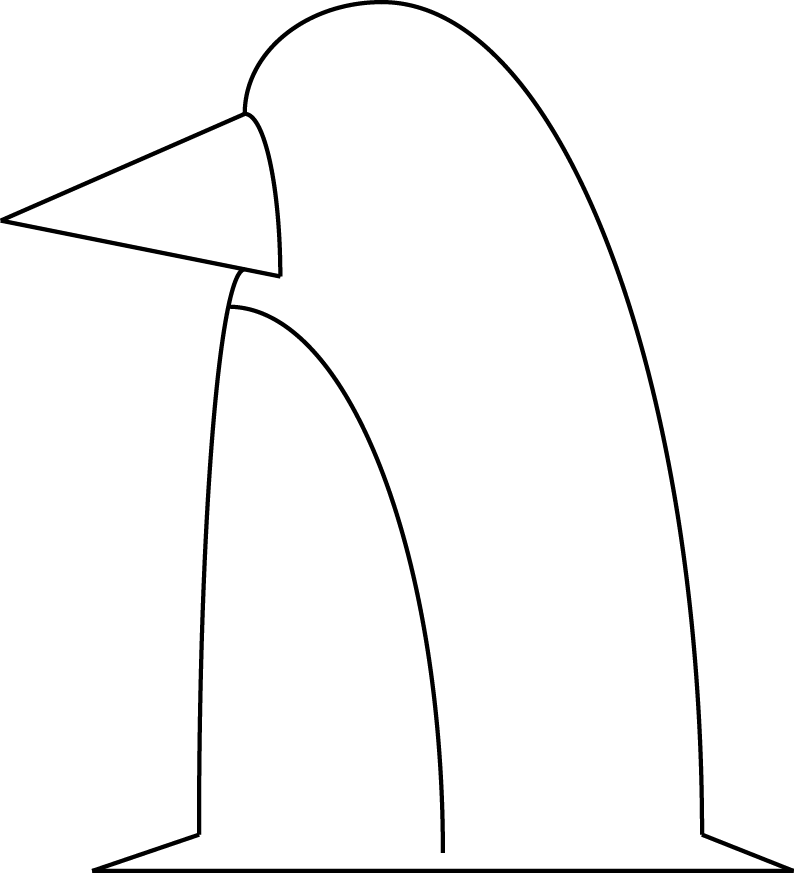
\includegraphics[width=\textwidth]{penguin}
%\end{subfigure}
%\caption{This is a penguin, filling the emptiness of this page until more text is available.}
%\label{penguin}
%\end{figure}

%Experimenting with cold atoms has become a major part of modern physical research and has let to new insights in the fields of quantum simulation and quantum information, shedding light also on other fields in physics from high energy to condensed matter. A vital set of techniques, enabeling such experiments is based on trapping, storing and cooling atoms with conservative forces, induced by the interaction of the dipole-moment with far detuned laser-light. A commonly used concept for preparing the investigated system is the optical lattice. Using interfering beams, that form a standing wave, a landscape of periodic potentials is created that can be used to resemble the lattice-structure in a solid cristal enabeling the simulation of many effects in many-body physics such as supercondctivity, superfuiditiy or Mott insulation. To actually perform experiments in such a potential-structure it is of vital importance to get information about the atoms behaviour while interacting in the lattice. This however is not a trivial problem, since the only possibility to get an insight into the state of the system is by driving atomic transitions and either collecting photons, showing the position of the atoms or using the absorbtion to get an inverse image of the cloud. These measurements are mostly done short periods after deactivating the trap-beams. While absorbtion imaging can in principle be done within the trap or lattice, it is not suitable to resolve low numbers of particles. fluorescence imaging on the other hand can be accurate enough to count single atoms but so far few approaches have been implemented, that are able to perform this technique inside the trap. A part of the issue is, that an atom that is excited for using its spontanious emission has a different induced dipole moment and reacts differently to the used lasers than the groundstate, that is initially trapped in the experiment. Depending on the atomic species, the trapping forces could be higher, lower or even repulsive in an excited state, rendering detection of enough fluorescence impossible without messing up the distribution inside the lattice or dissolving the cloud as a whole. On goal in our experiment is to use the fluorescence of the D2-line in Lithium-6 to image single sites in a multiwell-potential in an infrared dipole-trap. To achieve this it has to be investigated whether the excited state is still trapping and whether the trapping force is stron enough to hold the atoms long enough to collect enough spontanious radiation.
%\section{Outline}
%In this thesis the \textsc{ac}-Stark shift of the ground and the excited state of the atomic transition are calculated and tested in experiment. This enables the prediction of trap depths for each state and allows conclusions regarding the seeked fluorescence imaging inside dipole-traps. The thesis starts by giving a general overview about the experiment with its features and goals. The next part shortly describes the theoretic foundation of the atomic structure followed by a detailed analysis of the interaction of particles with electromagnetic waves, leading to the formulas later used to calculate the \textsc{ac}-Stark shift for the $2s_{1/2}$ and $2p_{3/2}$ states 